\documentclass[ignorenonframetext,xcolor=x11names]{beamer}

\definecolor{mun}{RGB}{134,38,51}
\definecolor{mun2}{RGB}{99,102,106}
%\definecolor{mun}{cmyk}{0,.3922,.2392,.1686}
\definecolor{code}{RGB}{0, 0, 128}
\definecolor{code}{gray}{0.95}

\mode<presentation>
{
%  \usetheme{boxes}
%  \usetheme{default}
%  \usetheme{Montpellier}
%  \usetheme{Singapore}
%   \usetheme{Rochester}
%  \usecolortheme{crane}
%  \usecolortheme{dolphin}
%  \usecolortheme{lily}
%  \usecolortheme{orchid}
  \usecolortheme{rose}
  \setbeamercovered{transparent}
%  \usefonttheme[onlymath]{serif}
  \setbeamercolor*{structure}{bg=mun,fg=mun}
  \setbeamercolor*{palette primary}{use=structure,fg=white,bg=structure.fg}
  \setbeamercolor*{palette secondary}{use=structure,fg=white,bg=structure.fg}
  \setbeamercolor*{palette tertiary}{use=structure,fg=white,bg=black}
  \setbeamercolor*{palette quaternary}{fg=white,bg=black}
  \setbeamercolor{section in toc}{fg=black,bg=white}
  \setbeamercolor{alerted text}{use=structure,fg=structure.fg!50!black!80!black}
  \setbeamercolor{titlelike}{parent=palette primary,fg=structure.fg!50!black}
  \setbeamercolor{frametitle}{bg=mun,fg=white}
  \setbeamercolor*{titlelike}{parent=palette primary}

  \setbeamercolor{normal text}{fg=black!90}
  \setbeamercolor{math text}{fg=black}
  \setbeamercolor{quote}{bg=gray!20}
  \setbeamercolor{quotation}{bg=gray!20}
  \setbeamerfont{cite}{size=\scriptsize}
  \setbeamerfont{quote}{size=\footnotesize}
  \setbeamerfont{quotation}{size=\footnotesize}
  \setbeamercolor{red text}{fg=red!75!black}
  \setbeamertemplate{bibliography item}[triangle]
  \setbeamertemplate{enumerate item}[square]
  \setbeamertemplate{blocks}[rounded][shadow=true]
  \setbeamertemplate{navigation symbols}{}
  \setbeamertemplate{footline}[frame number]
}
\usepackage{tcolorbox}
\usepackage{amsmath}
\usepackage{physics}
\usepackage{pgf}
\usepackage[english]{babel}
\usepackage[latin1]{inputenc}
\usepackage{times}
\usepackage[T1]{fontenc}
\usepackage{multicol}
\usepackage{multirow}
\usepackage{fancyvrb}
\usepackage{tabularx}
\usepackage{amsmath}
\usepackage{bbm}
\usepackage{alltt}
\usepackage{hyperref}
\hypersetup{
    colorlinks=true,
    linkcolor=blue,
    filecolor=magenta,      
    urlcolor=blue,
}
\usepackage{minted}
\newminted{cypher}{autogobble,bgcolor=code,breakbytoken,frame=single,framesep=3pt}
\newminted{R}{autogobble,bgcolor=code,breakbytoken,frame=single,framesep=3pt}
\newminted{text}{autogobble,bgcolor=code,breakbytoken,frame=single,framesep=3pt}
\newminted{sql}{autogobble,bgcolor=code,breakbytoken,frame=single,framesep=3pt}
\newminted{bash}{autogobble,bgcolor=code,breakbytoken,python3,frame=single,framesep=3pt}
\newminted{xml}{autogobble,bgcolor=code,breakbytoken,python3,frame=single,framesep=3pt}
\newminted{python}{bgcolor=code,breakbytoken,python3,frame=single,framesep=3pt}
\newminted{html}{autogobble,bgcolor=code,breakbytoken,frame=single,framesep=3pt}
\newminted{js}{autogobble,bgcolor=code,breakbytoken,frame=single,framesep=3pt}
\AtBeginEnvironment{minted}{%
  \renewcommand{\fcolorbox}[4][]{#4} \scriptsize}
\AtEndEnvironment{minted}{%
  \normalsize}

%\newcommand{\Pr}{\operatorname{Pr}}
\newcommand{\argmax}{\operatorname*{argmax}}
\newcommand{\argmin}{\operatorname*{argmin}}
\newcommand{\Ident}{\operatorname{I}}

\author % (optional, use only with lots of authors)
{Joerg Evermann}
% - Give the names in the same order as the appear in the paper.
% - Use the \inst{?} command only if the authors have different
%   affiliation.

\institute%[Universities of Somewhere and Elsewhere] % (optional, but mostly needed)
{
  Faculty of Business Administration\\
  Memorial University of Newfoundland \\ 
  \texttt{jevermann@mun.ca} 
}

\date{}

\pgfdeclareimage[width=1.5cm]{university-logo}{../MUN_LOGO_CMYK}
\logo{\pgfuseimage{university-logo}}

% If you wish to uncover everything in a step-wise fashion, uncomment
% the following command: 

%\beamerdefaultoverlayspecification{<+->}

 
\title{Business 4720 - Class 9}

\subtitle{Process Analytics}

\begin{document}

\begin{frame}{}
  \titlepage
  \footnotesize
  \begin{center}

\includegraphics[height=.5in]{../by-nc.png}

Unless otherwise indicated, the copyright in this material is owned by Joerg Evermann. This material is licensed to you under the \href{https://creativecommons.org/licenses/by-nc/4.0/}{Creative Commons by-attribution non-commercial license (CC BY-NC 4.0)}
\end{center}

\end{frame}

\section{Introduction}

\begin{frame}{This Class}

\begin{block}{What You Will Learn:}
\begin{itemize}
  \item Introduction to Process Data
  \item Introduction to Process Analytics
  \begin{itemize}
     \item Process Discovery
     \item Process Conformance Analysis
     \item Process Performance Analysis
  \end{itemize}
\end{itemize}
\end{block}
\end{frame}

\section{BPMN}

\begin{frame}{Business Processes}
\begin{itemize}
   \item Sequence of activities in a defined order
   \item Models describe processes
   \item Typically related to the processing of one type of business object
   \begin{itemize}
      \item e.g. an order, a prescription, a complaint, etc.
   \end{itemize}
   \item Standard notation: BPMN (''Business Process Modeling Notation'')
\end{itemize}

\begin{block}{Basic BPMN}
\begin{itemize}
   \item Events (circles)
   \item Activities (boxes)
   \item Gateways (diamonds)
   \begin{itemize}
      \item Exclusive (''X'') split and merge
      \item Parallel (''+'') split and merge
      \item Inclusive (''O'') split and merge
   \end{itemize}
\end{itemize}
\end{block}
\end{frame}

\begin{frame}{BPMN Example Process Model}
\centering
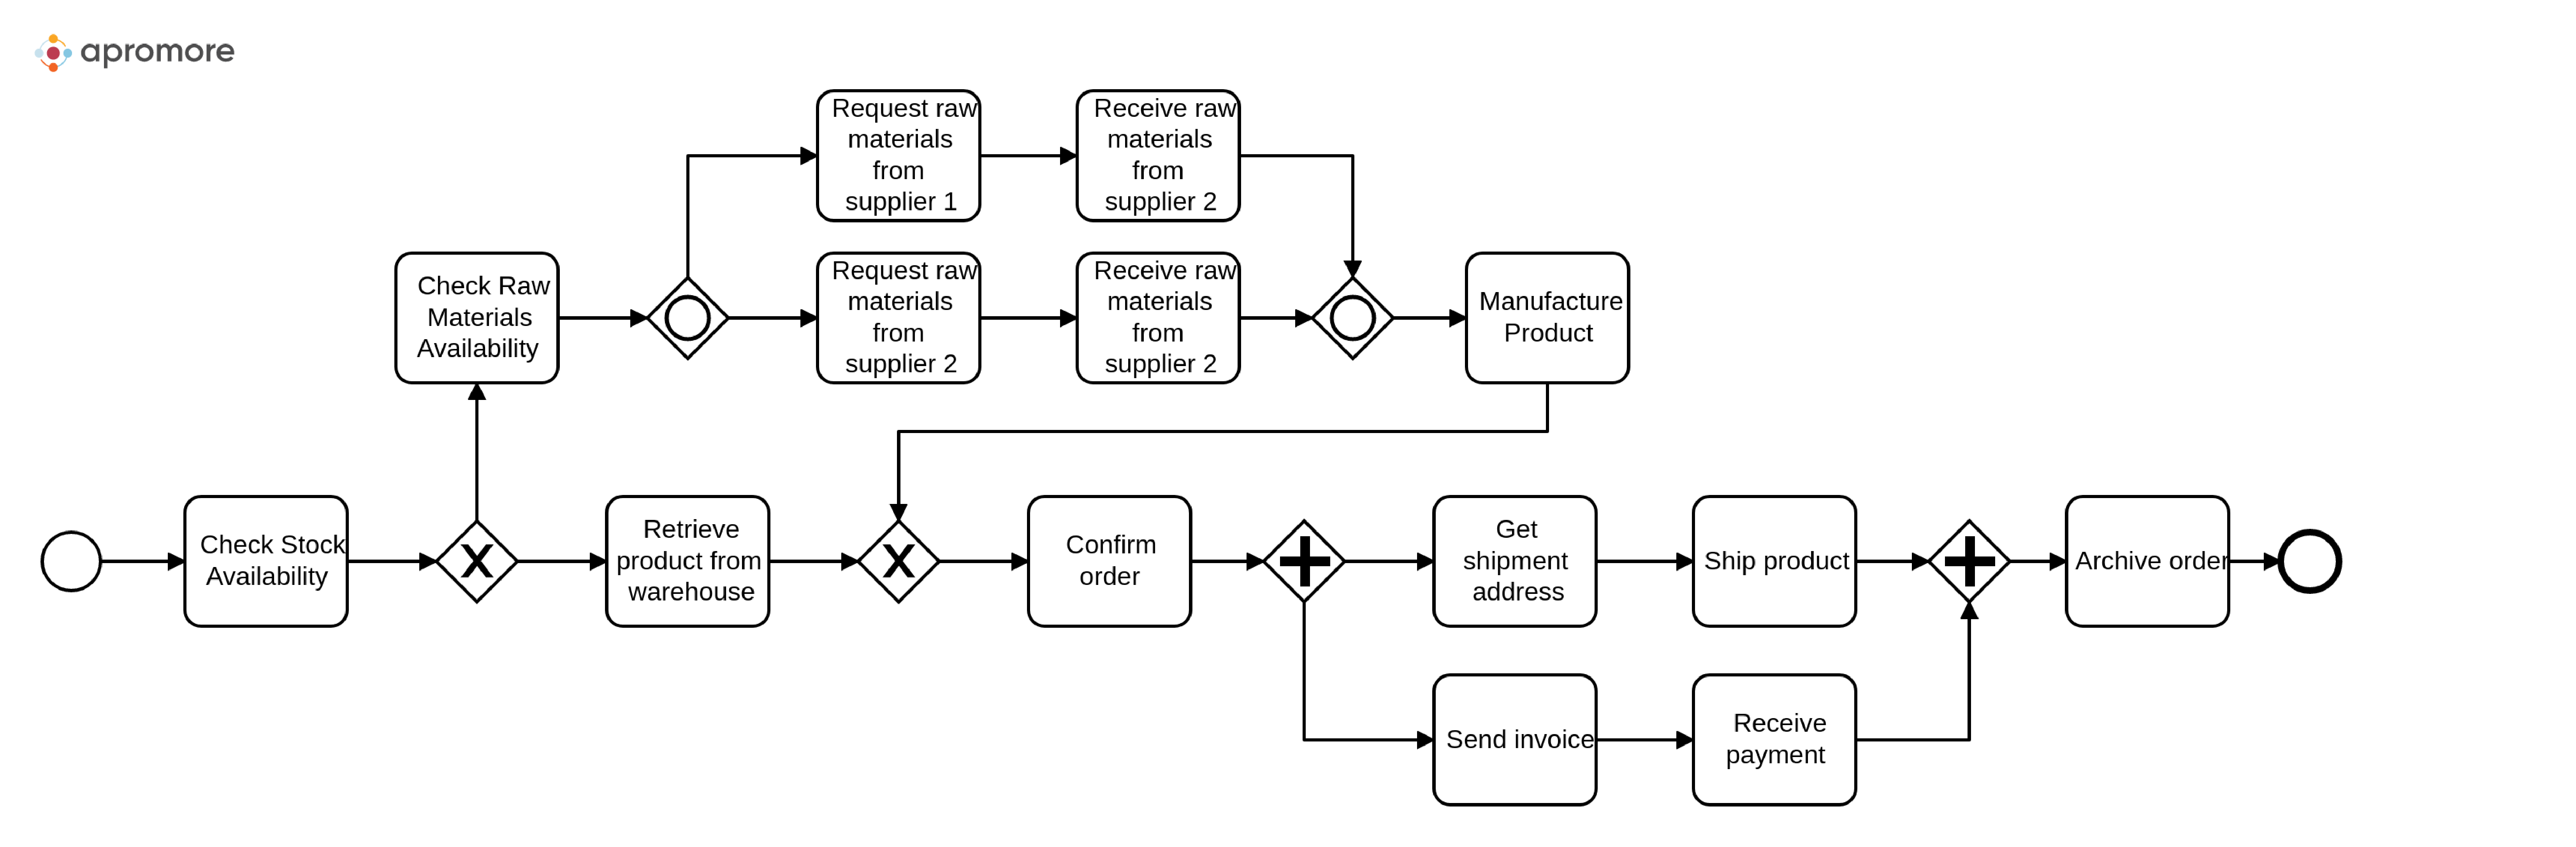
\includegraphics[width=1.15\textwidth]{Figure3.12.pdf}
\end{frame}

\begin{frame}{Business Process Instances and Process Data}
\begin{block}{Case}
\begin{itemize}
   \item One instance of a business process
   \item Related to one particular business object (e.g. order 123, prescription R456, complaint C6789, etc.)
\end{itemize}
\end{block}
\begin{block}{Trace}
\begin{itemize}
   \item Event data sequence for one case
   \item May includes attributes for the case and for each event
   \item May include resource information for each event
   \item May include timestamps for events
\end{itemize}
\end{block}
\begin{block}{Event Log}
\begin{itemize}
   \item Set of traces for one process
   \item May include incomplete cases, may be sampled, etc.
\end{itemize}
\end{block}
\end{frame}

\begin{frame}{Activity Lifecycle -- Example}
\centering

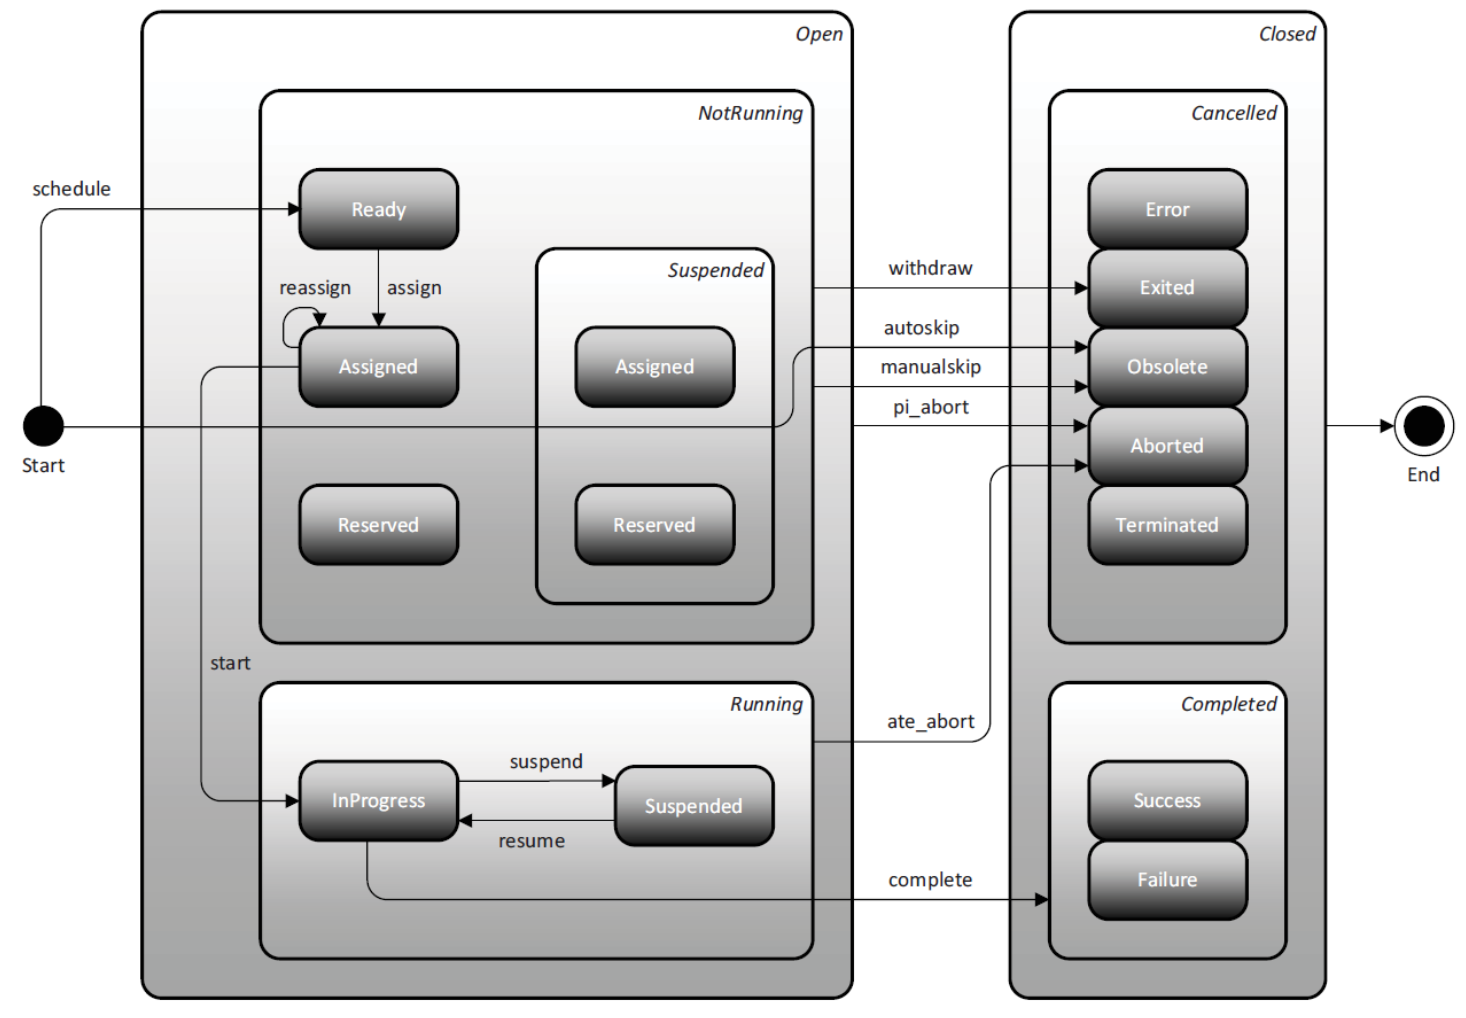
\includegraphics[height=2.25in]{screen1.png}

\scriptsize\url{https://www.tf-pm.org/resources/xes-standard/about-xes/standard-extensions/lifecycle/standard}
\normalsize
\end{frame}

\begin{frame}{Event Log Data}
\begin{block}{Sources}
\begin{itemize}
  \item Process aware information systems
  \item Web server data
  \item \ldots
\end{itemize}
\end{block}
\begin{block}{Formats}
\begin{itemize}
   \item CSV (one line per event)
   \item MXML (older XML format)
   \item XES (''eXtensible Event Stream'') (current XML format)
\end{itemize}
\end{block}
\begin{block}{Challenges}
\begin{itemize}
   \item Event correlation from multiple systems
   \item Noise, incompleteness
   \item Timestamping, batch processing
   \item Abstraction levels
\end{itemize}
\end{block}
\end{frame}

\begin{itemize}
   \item Not all lifecycle transition captured in event log; typically only ''complete'', or ''start'' and ''complete''
\end{itemize}
\end{frame}

\begin{frame}{Process Analytics}
\centering
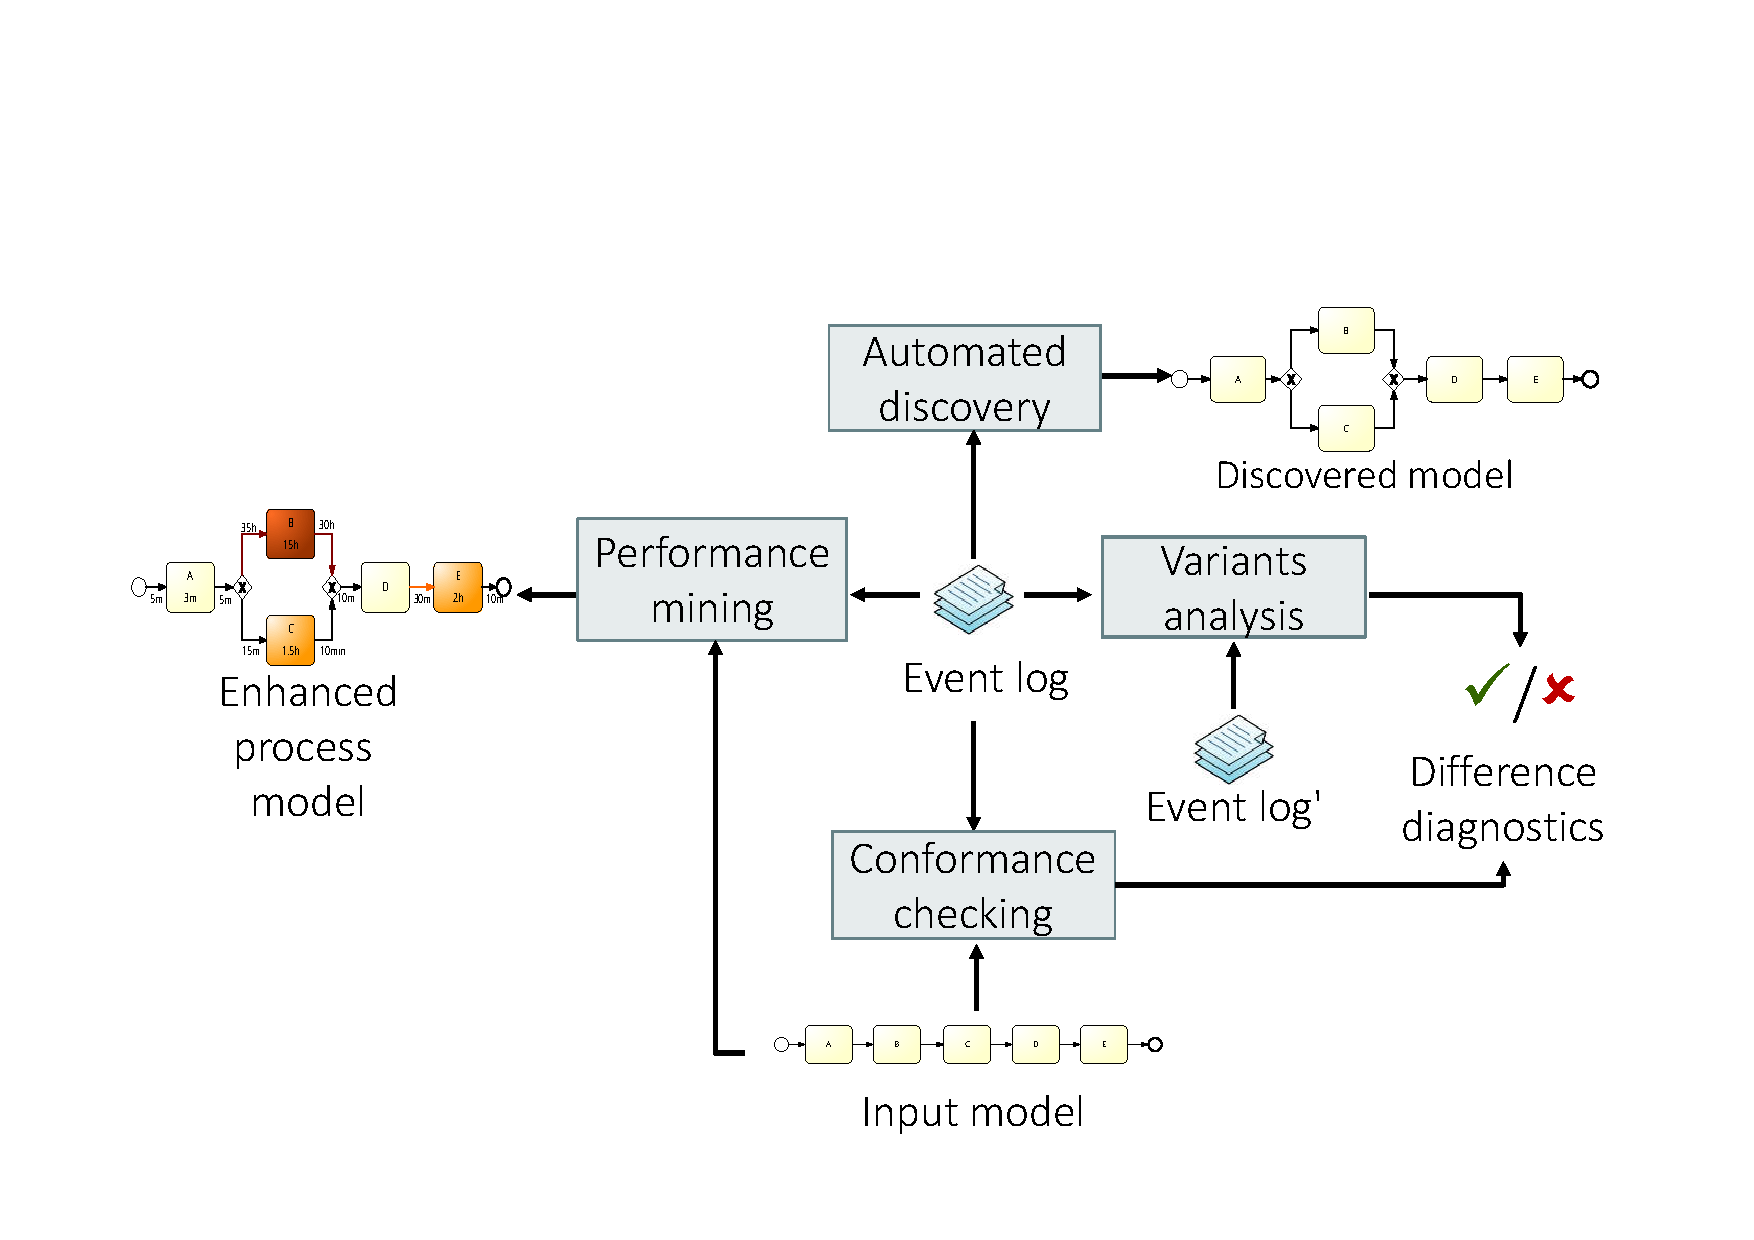
\includegraphics[width=.9\textwidth]{Chapter-11-Figure-03.pdf}\\
\vspace{3mm}\hrule\vspace{2mm}
\scriptsize{Source: Marlon Dumas, Marcello La Rosa, Jan Mendling, Hajo A. Reijers (2018) ''Fundamentals of Business Process Management'', 2nd edition, Springer Verlag, Germany}
\end{frame}

\begin{frame}{Process Analytics}
\begin{block}{Purpose}
\begin{itemize}
   \item Discover actual operations
   \item Check actual process against desired process
   \item Identify operational (performance) problems
   \item Improve operational processes
   \item External compliance analysis and reporting
   \item Identify implicit or de-facto organizational groups and relationships 
   \item Support, reinforce, or break organizational relationships
\end{itemize}
\end{block}
\end{frame}

\begin{frame}{Process Analytics in R}
\begin{block}{BupaR}
\begin{itemize}
   \item Hasselt University
   \item Open source R library
   \item Development since 2020
   \item Process visualization (DFG)
   \begin{itemize}
      \item Frequencies metrics
      \item Performance metrics
   \end{itemize}
   \item Control flow analysis
   \item Rule-based conformance analysis
   \item Performance metrics
   \item Organizational analysis
\end{itemize}
\end{block}
\vspace{.5\baselineskip}
\url{https://bupar.net/}

\end{frame}

\begin{frame}{Process Analytics in Python}
\begin{block}{PM4PY}
\begin{itemize}
   \item Fraunhofer Institute for Applied Information Technology
   \item Open source python package, since 2018
   \item Process discovery
   \begin{itemize}
       \item \emph{Techniques}: Inductive miner, Heuristics miner, \ldots
   \end{itemize}
   \item Conformance checking
   \begin{itemize}
       \item \emph{Techniques}: Token-based replay, Cost-based alignment, \ldots
   \end{itemize}
   \item Log--Model Comparison
   \begin{itemize}
       \item \emph{Metrics}: Fitness, Precision, Generalization, Complexity, \ldots
   \end{itemize}
   \item Decision mining
   \item Trace clustering
   \item LTL checking
   \item Social network discovery
\end{itemize}
\end{block}
\vspace{.5\baselineskip}
\url{https://processintelligence.solutions/pm4py}

\end{frame}

\begin{frame}[fragile]{PM4PY Basics}
Read a CSV dataset:
\footnotesize
\begin{pythoncode}
import pandas as pd
import pm4py

# Load the event log and parse date columns
log = pd.read_csv('https://evermann.ca/busi4720/\
   PurchasingExample.csv', 
   parse_dates=['Start Timestamp', \
      'Complete Timestamp'], 
   infer_datetime_format=True)

# Tell PM4PY about which columns represent case ID,
# activity name, and timestamp. Case ID and activity
# names must be string type
log['case:concept:name']=log['Case ID'].astype('string')
log['concept:name']=log['Activity'].astype('string')
log['time:timestamp']=log['Complete Timestamp']
log['org:resource']=log['Resource']
\end{pythoncode}

\end{frame}

\begin{frame}[fragile]{PM4PY Basics}
%Continued from previous slide \ldots
%\footnotesize
%\begin{pythoncode}
%# Convenient but deprecated:
%# Tell PM4PY which columns are case_id, 
%# activity_key and timestamp
%log = pm4py.format_dataframe(log, 
   %case_id='Case ID', 
   %activity_key='Activity', 
   %timestamp_key='Complete Timestamp')   
%\end{pythoncode}
%\normalsize
Reading an XES file is easy:
\footnotesize
\begin{pythoncode}
log2 = pm4py.read_xes('BPI_Challenge_2012.xes.gz')
\end{pythoncode}
\end{frame}

\begin{frame}[fragile]{PM4PY Basic Statistics}
\footnotesize
\begin{pythoncode}
num_cases = len(log['Case ID'].unique())
num_events = log.shape[0]

pm4py.get_start_activities(log)
pm4py.get_end_activities(log)

pm4py.get_all_case_durations(log)

# Useful only or XES-based event logs
pm4py.get_event_attributes(log)
pm4py.get_trace_attributes(log)
\end{pythoncode}
\end{frame}

%\begin{frame}[fragile]{PM4PY Statistics on Dataframes}
%\footnotesize
%\begin{pythoncode}
%log['activity_duration']= \
   %log['Complete Timestamp']-log['Start Timestamp']

%tmp=log.groupby('case:concept:name')['time:timestamp']\
   %.apply(lambda g: g.max() - g.min()).reset_index() \
   %.rename({'time:timestamp':'case_duration'}, axis=1)
%log=log.merge(tmp)

%tmp=log.groupby('case:concept:name')['concept:name']\
   %.count().reset_index() \
   %.rename({'concept:name':'activity_count', axis=1})
%log=log.merge(tmp)

%tmp=log.groupby('case:concept:name')['concept:name']\
   %.nunique().reset_index() \
   %.rename(columns={'concept:name': \
                    %'unique_activity_count'},axis=1)
%log=log.merge(tmp)
%\end{pythoncode}
%\end{frame}

\begin{frame}[fragile]{PM4PY Basic Statistics}
\begin{itemize}
   \item Variants are sets of traces with the same sequence of events
\end{itemize}
\footnotesize
\begin{pythoncode}
pm4py.get_variants(log)

# Split the log into sub-logs
for variant, subdf in \
pm4py.split_by_process_variant(log):
    print(variant)
    print(subdf)  
\end{pythoncode}
\end{frame}

\begin{frame}[fragile]{Process Discovery -- DFG}
\begin{block}{Directly-Follows Graph \\ (Dependency Graph) (Process Map)}
\begin{itemize}
   \item Shows how often one activity directly follows another
\end{itemize}
\end{block}
\footnotesize
\begin{pythoncode}
dfg, start, end = pm4py.discover_dfg(log)

pm4py.view_dfg(dfg, start, end, rankdir='LR')

pm4py.save_vis_dfg(dfg=dfg,
    start_activities=start, 
    end_activities=end, 
    file_path='dfg.png', rankdir='TB')
\end{pythoncode}
\end{frame}

\begin{frame}{Process Discovery}
\centering
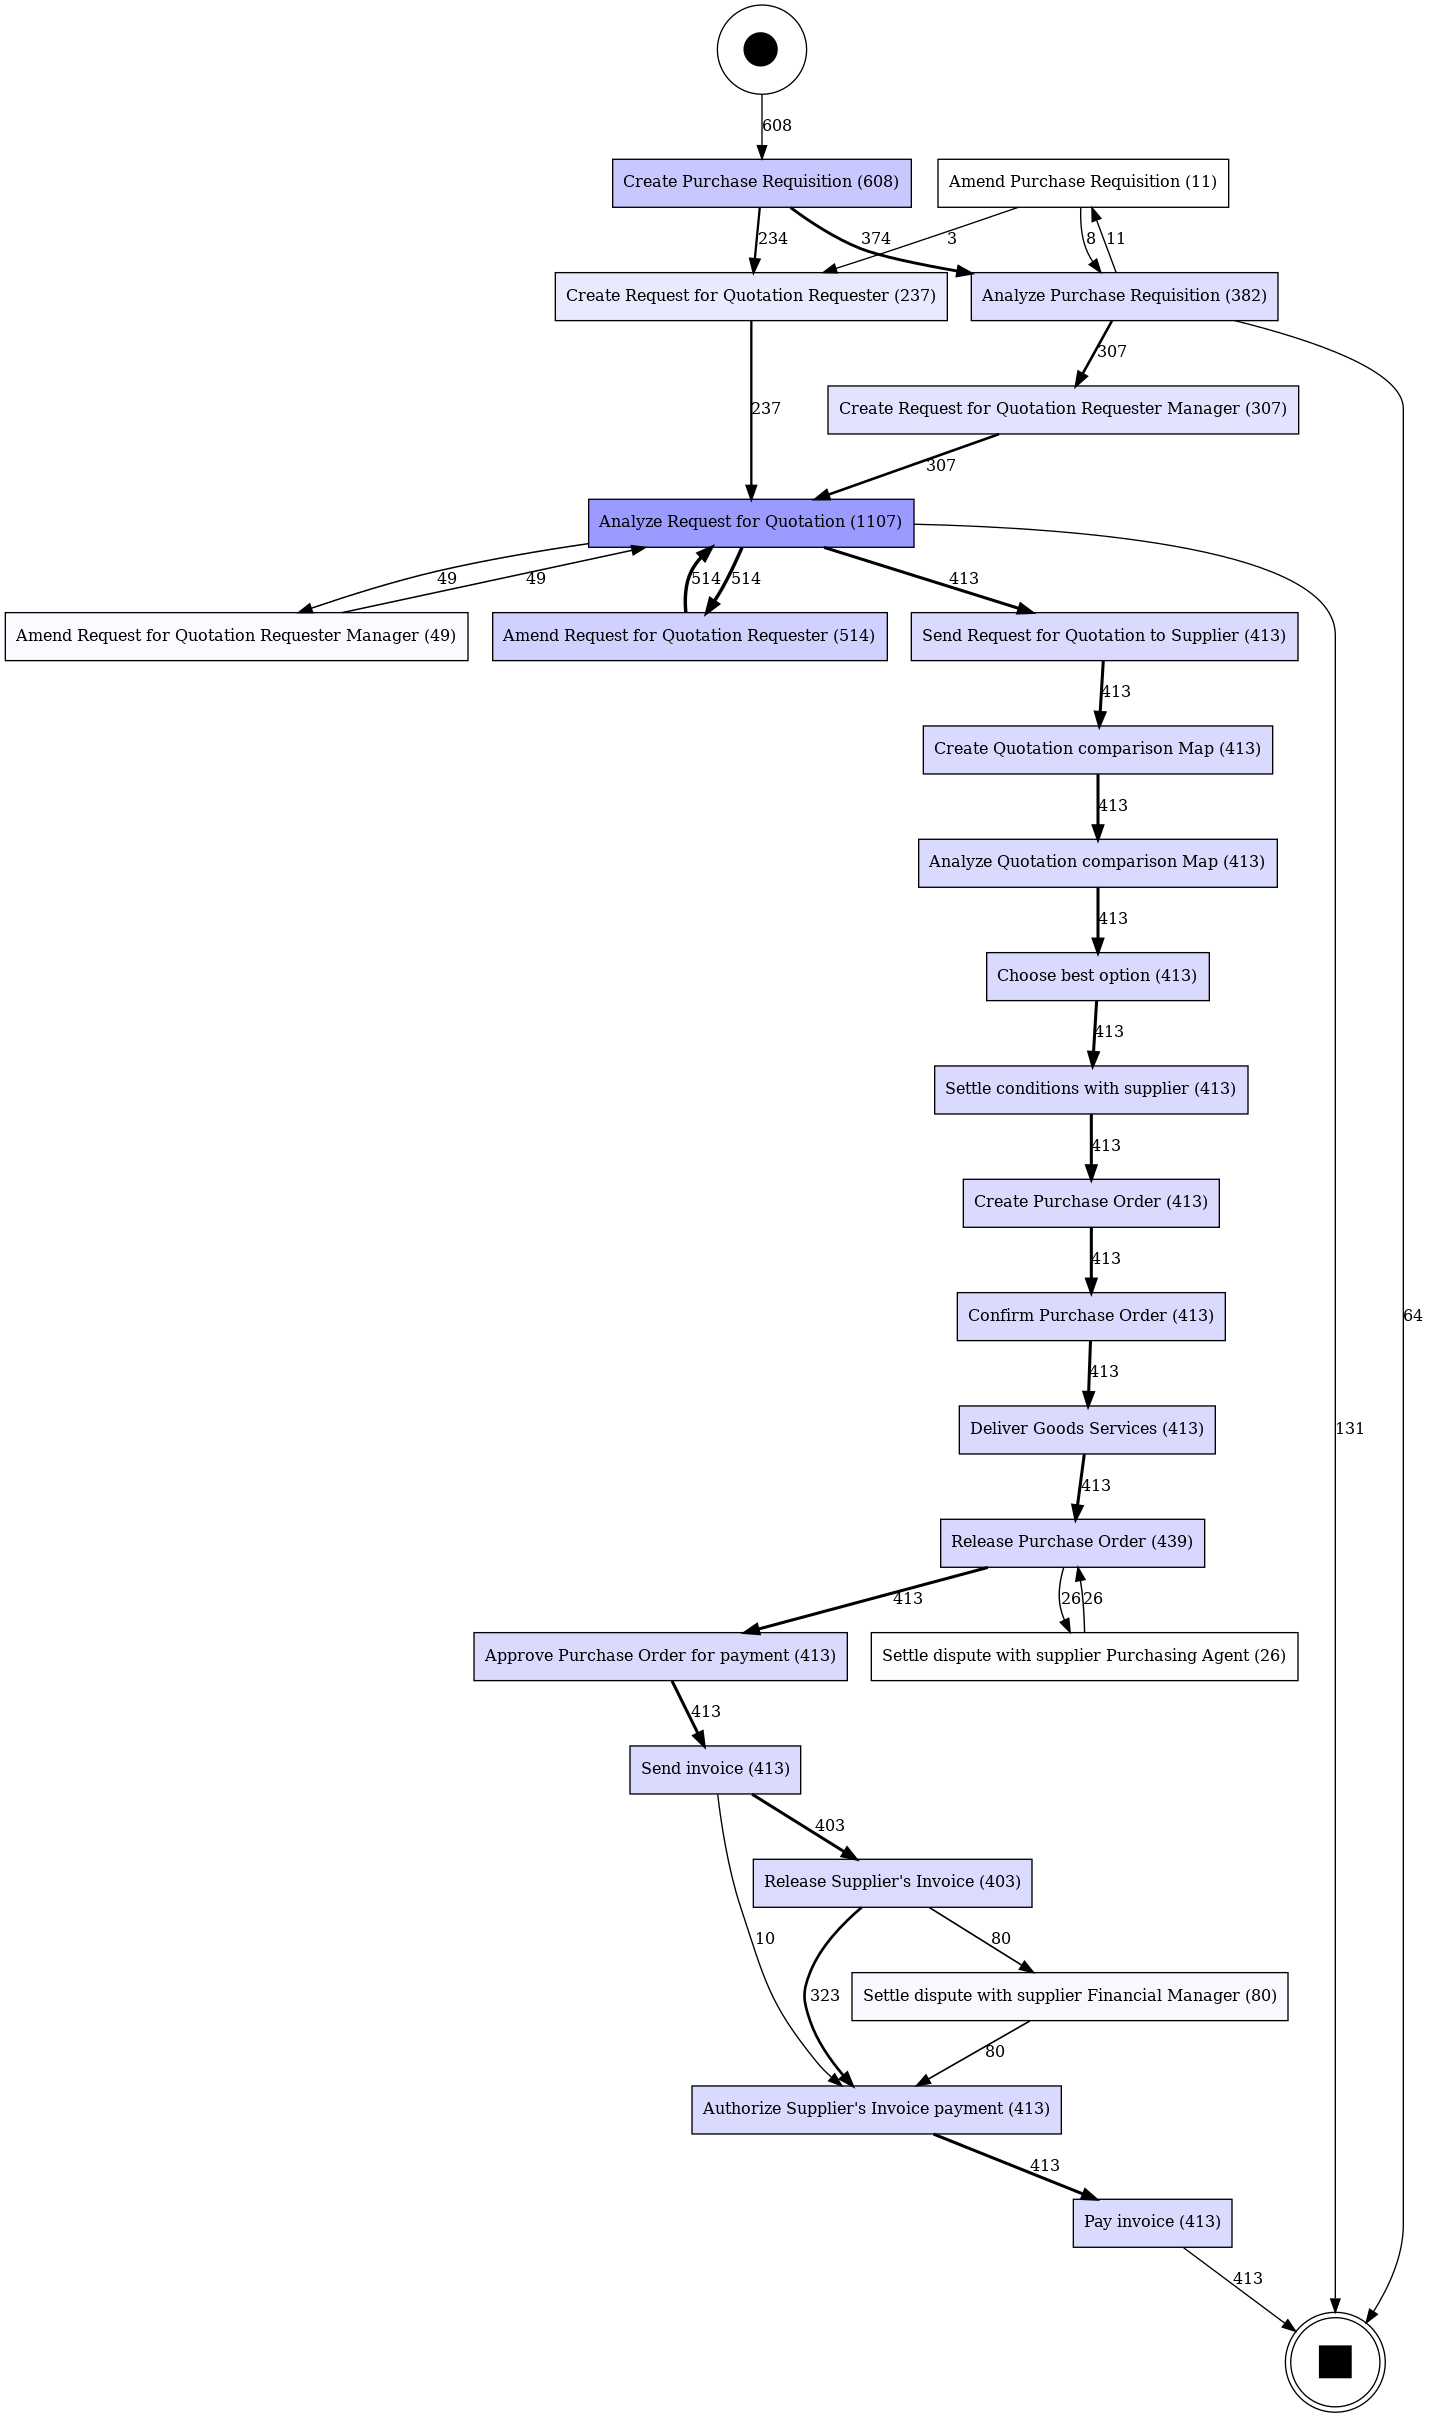
\includegraphics[width=\textwidth]{dfg.png}
\end{frame}

\begin{frame}{Process Discovery -- Inductive Miner}
\begin{block}{Principles}
\begin{itemize}
   \item Identifies subsets of activities by repeatedly ''cutting'' the DFG
   \item Filter infrequent activities to deal with noise
   \item Mines a process tree that can be transformed to BPMN
\end{itemize}
\end{block}
\end{frame}

\begin{frame}{Process Discovery -- Inductive Miner}
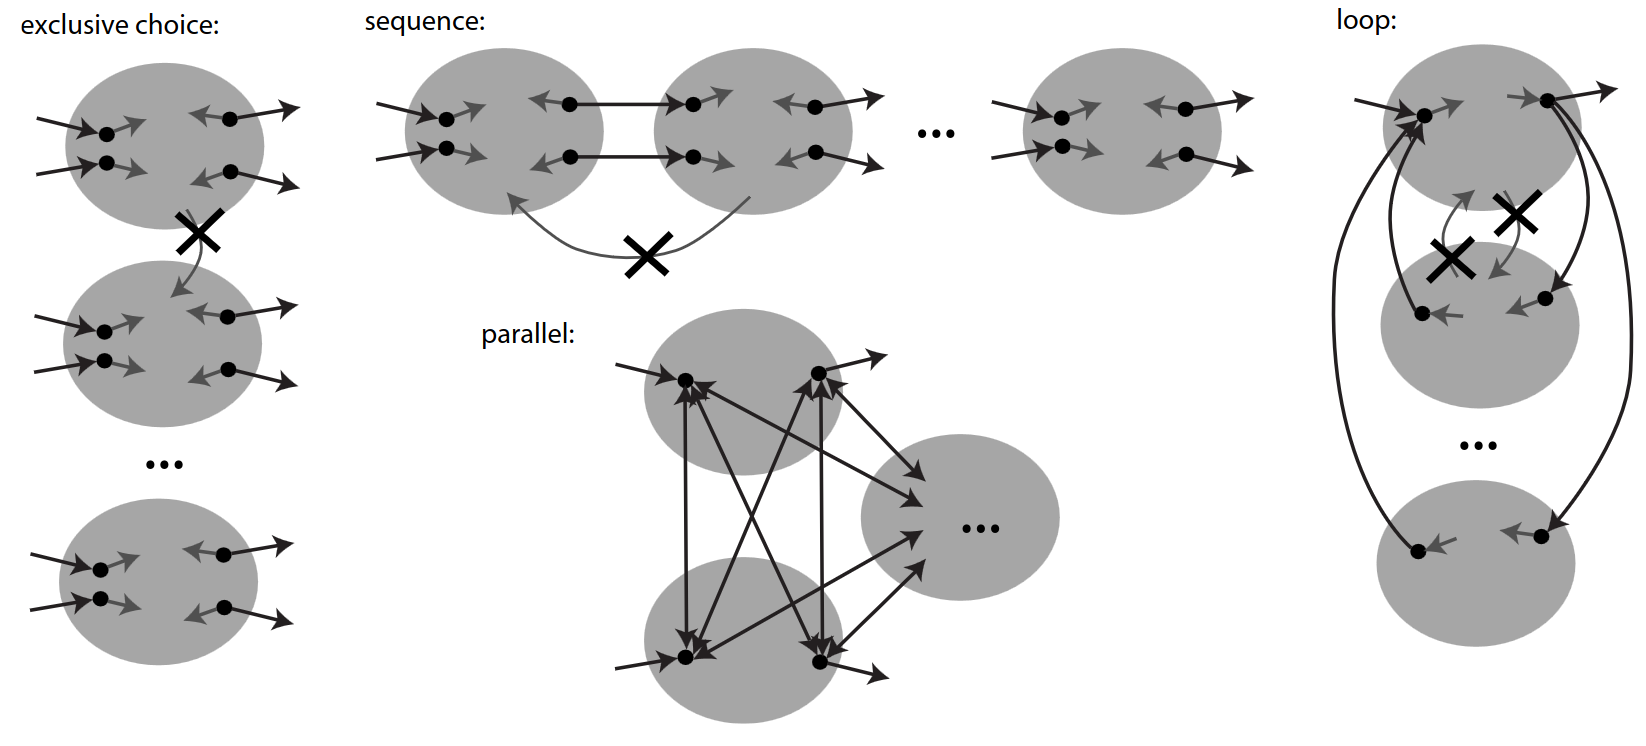
\includegraphics[width=\textwidth]{screen2.png}
\tiny 
Source: Leemans, S.J.J., Fahland, D., van der Aalst, W.M.P. (2013). Discovering Block-Structured Process Models from Event Logs - A Constructive Approach. In: Colom, JM., Desel, J. (eds) Application and Theory of Petri Nets and Concurrency. PETRI NETS 2013. Lecture Notes in Computer Science, vol 7927. Springer, Berlin, Heidelberg.
\end{frame}

\begin{frame}[fragile]{Process Discovery -- Inductive Miner}
\footnotesize
\begin{pythoncode}
bpmn_model = \
    pm4py.discover_bpmn_inductive(log, 
        noise_threshold=0.5)

pm4py.view_bpmn(bpmn_model, rankdir='LR')

pm4py.save_vis_bpmn(bpmn_model, 
   file_path='bpmn.png', rankdir='TB')
\end{pythoncode}
\end{frame}

\begin{frame}{Process Discovery -- Inductive Miner}
\centering
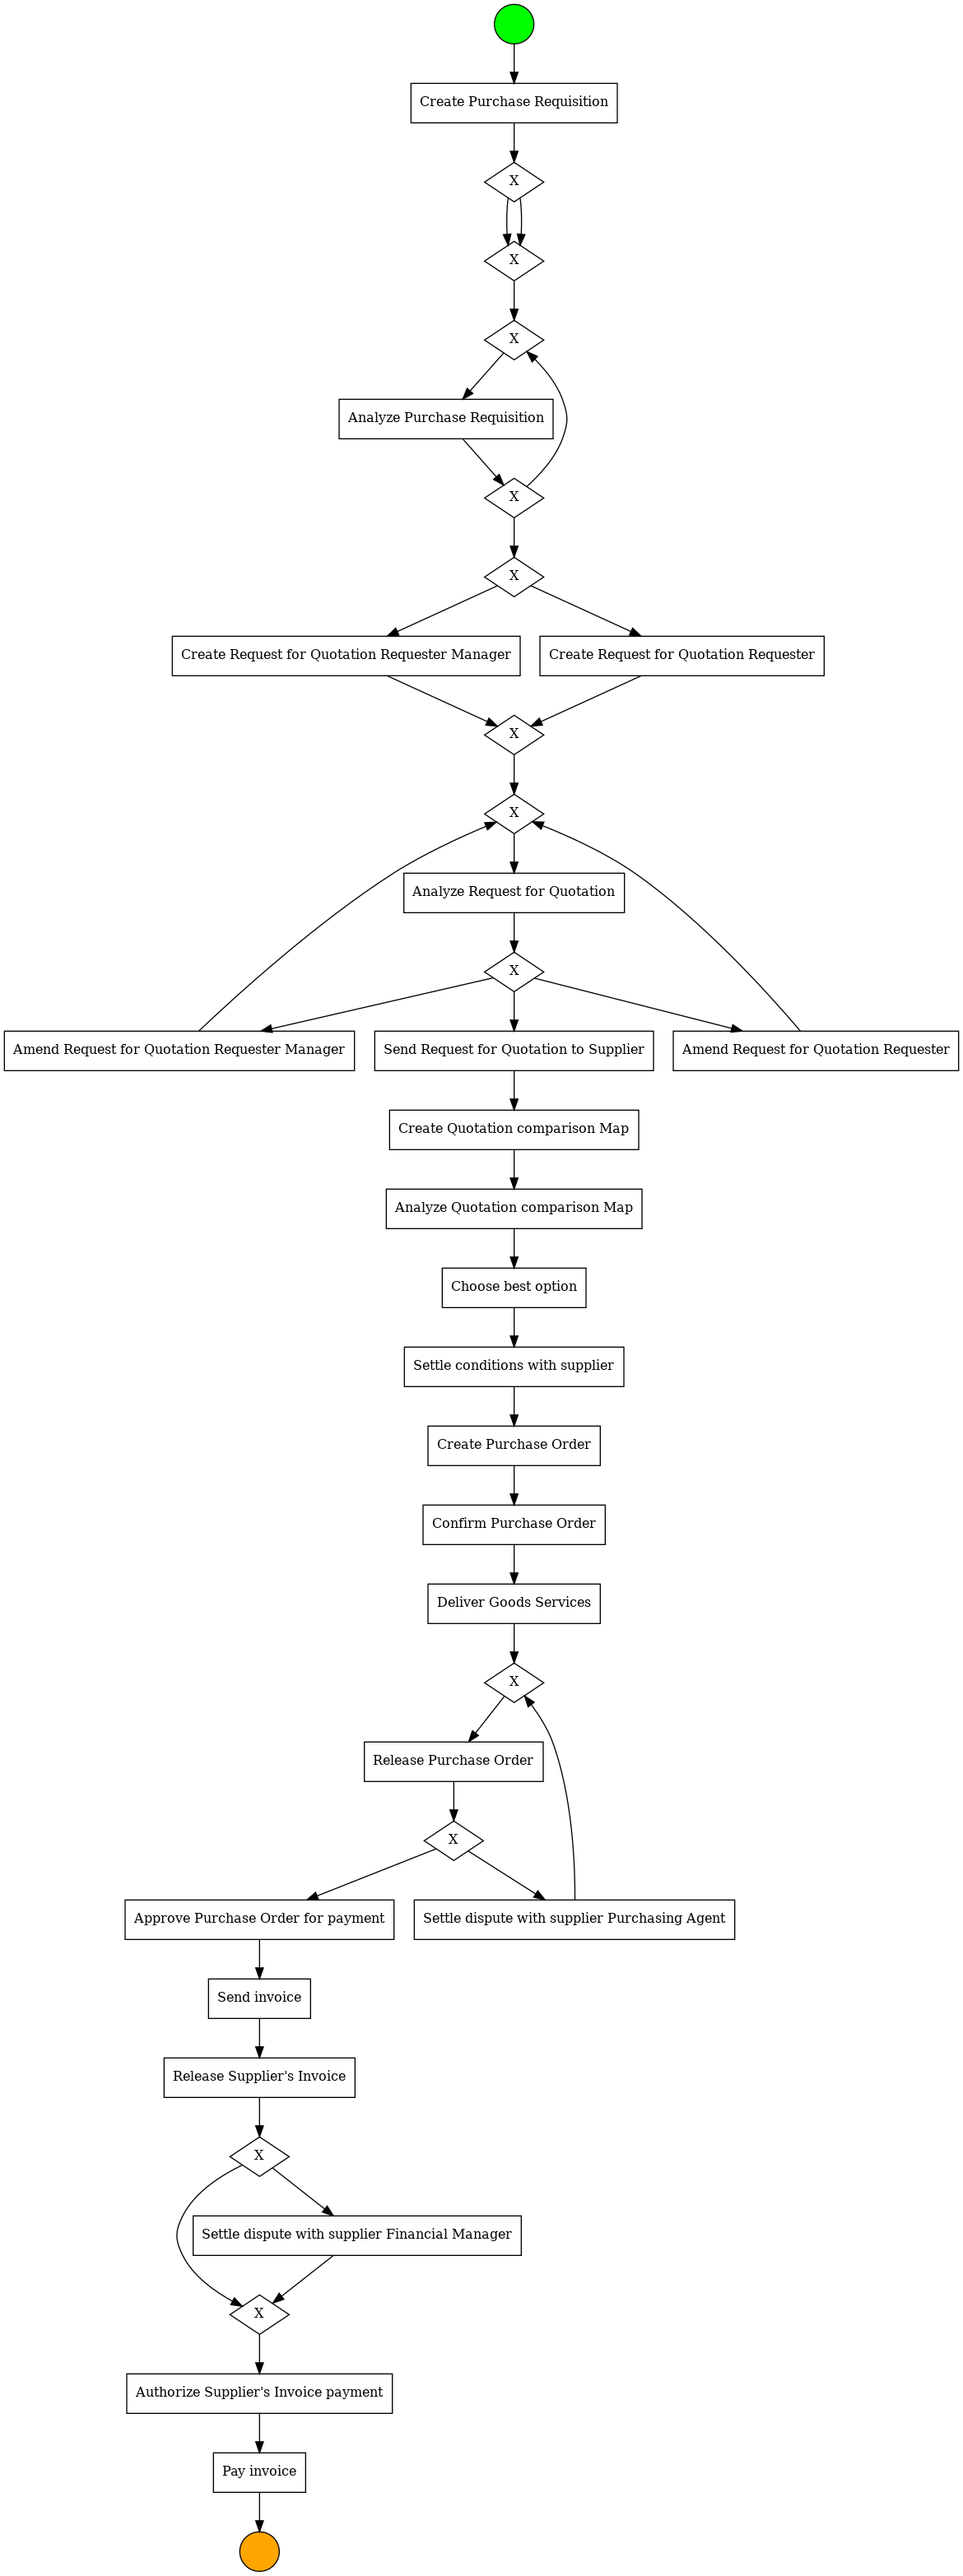
\includegraphics[width=.8\textwidth]{bpmn.png}
\end{frame}

\begin{frame}{Process Discovery -- Heuristics Net}
\begin{block}{Principles}
\begin{itemize}
   \item Remove noise by frequency threshold on dependency graph
   \item Identifies loops of length 1 and length 2
   \item Identifies long-distance dependencies
   \item Removes non-observable activities
\end{itemize}
\end{block}

\begin{block}{Frequencies in DFG}
\begin{align*}
a \Rightarrow b = \left( \frac{
| a > b| - |b > a|}{
| a > b| + |b > a| + 1}\right)
\end{align*}
\end{block}
\end{frame}

\begin{frame}[fragile]{Process Discovery -- Heuristics Net}
\footnotesize
\begin{pythoncode}
petri_net, initial_marking, final_marking = \
    pm4py.discover_petri_net_heuristics(log, 
        dependency_threshold=0.6,
        and_threshold=0.65,
        loop_two_threshold=0.4)
        
pm4py.view_petri_net(petri_net)
        
bpmn_model2 = pm4py.convert_to_bpmn(
    petri_net, initial_marking, final_marking)
    
pm4py.view_bpmn(bpmn_model2)
pm4py.save_vis_bpmn(bpmn_model2, 
    'bpmn2.png', rankdir='TB')
\end{pythoncode}
\end{frame}

\begin{frame}{Process Discovery -- Heuristics net}
\centering
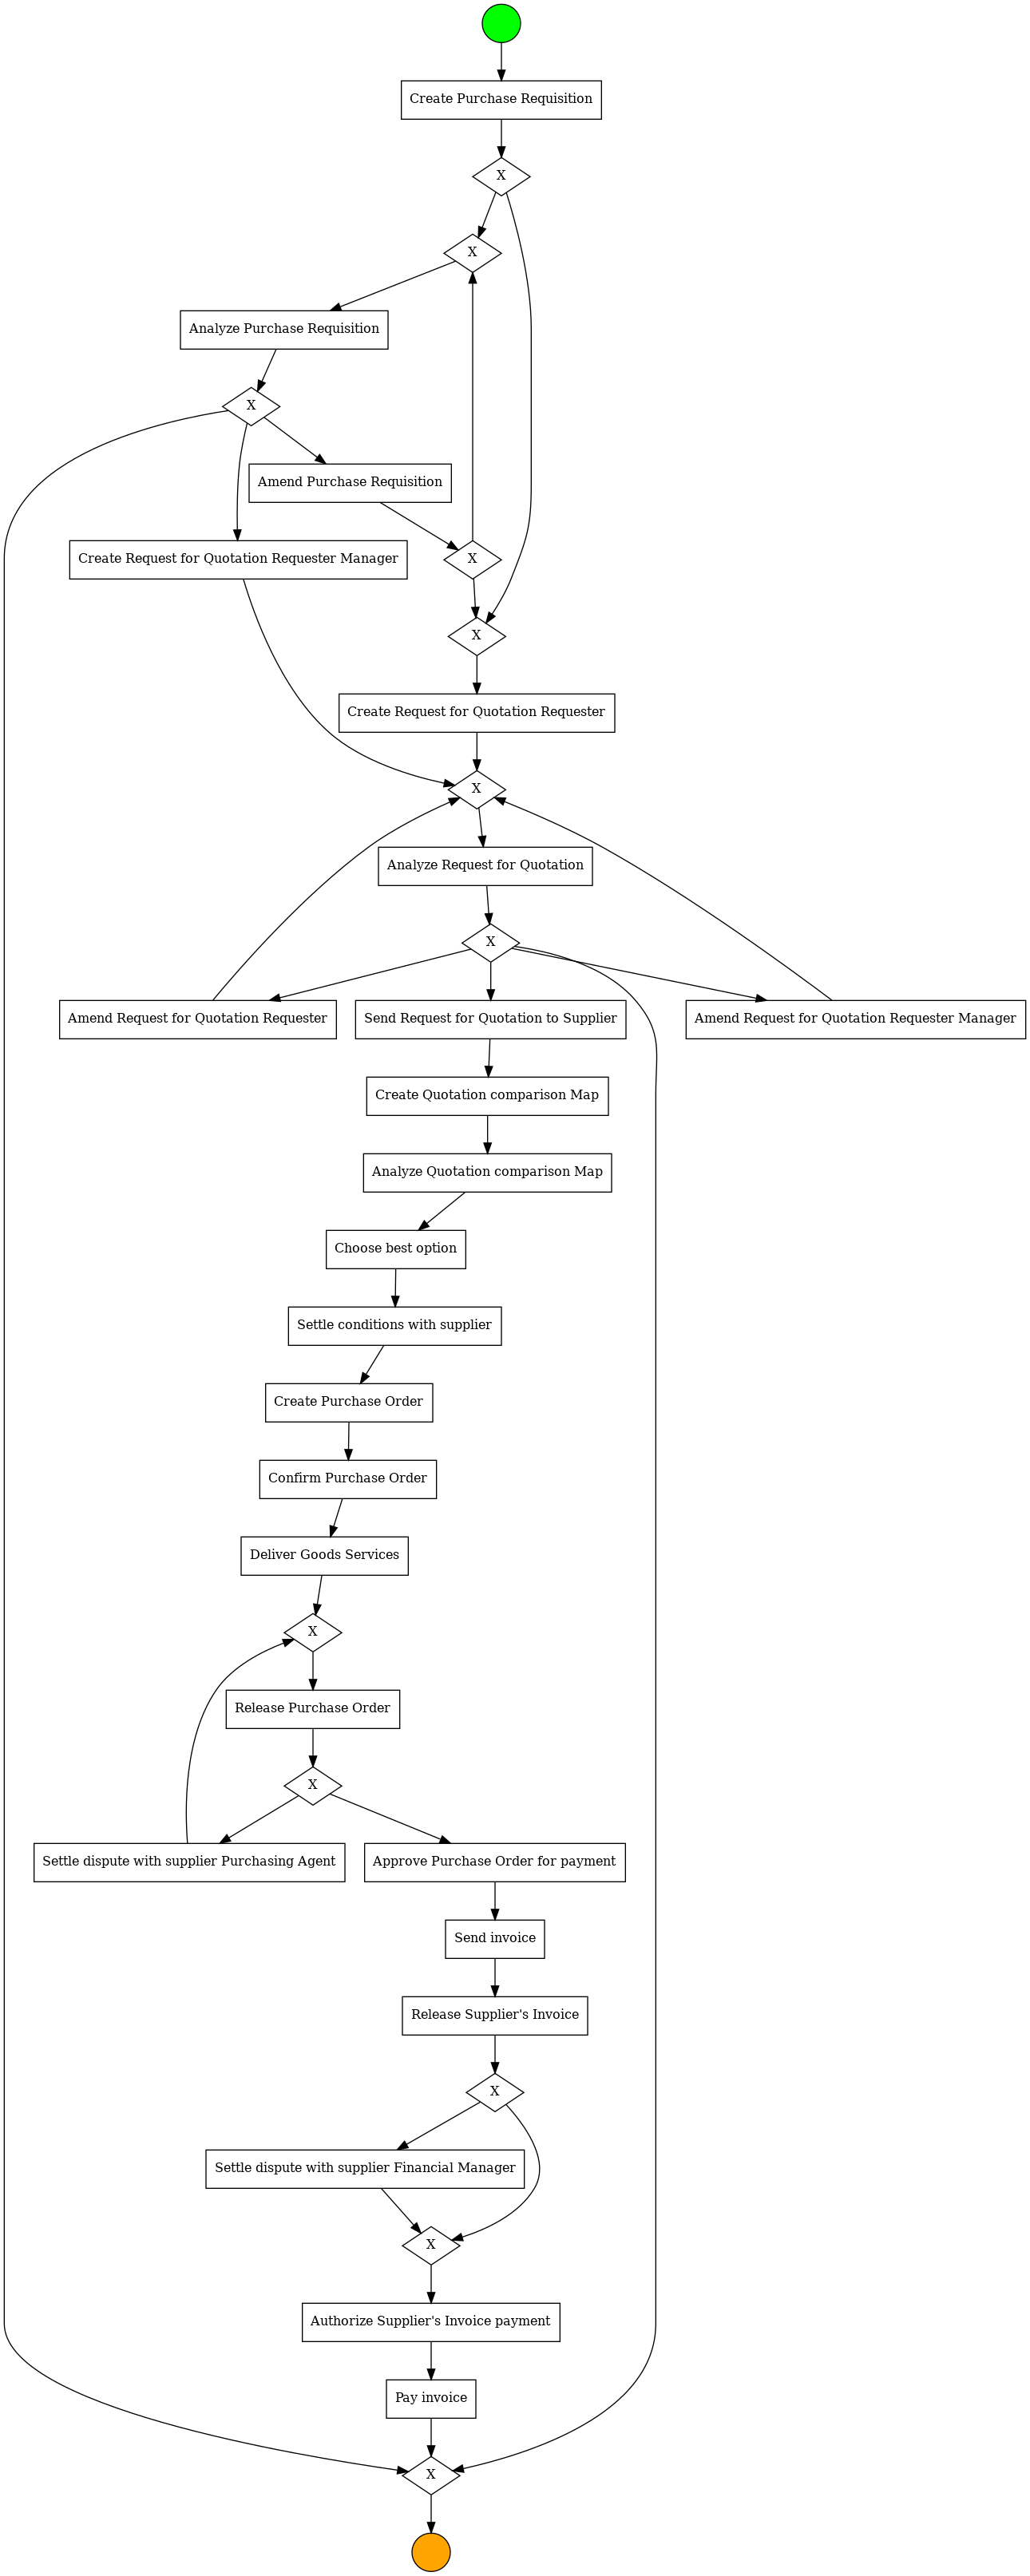
\includegraphics[width=.8\textwidth]{bpmn2.png}
\end{frame}

\begin{frame}{Process Discovery}
\begin{block}{Quality of Discovered Models}
\begin{itemize}
   \item \textbf{Fitness}: Can the model generate all traces in log?
   \item \textbf{Precision}: Does the model only generate traces in log?
   \item \textbf{Generalization}: Can the model generalize to ''sensible'' traces not seen in log?
   \item \textbf{Complexity}: Is the model too complex to understand?
\end{itemize}
\end{block}
\end{frame}

\begin{frame}{Fitness \& Precision}
\begin{block}{Token-Based Replay}
\begin{itemize}
   \item Replays each trace of an event log on a process model
   \item Discovers missing and surplus tokens, i.e. model activities that cannot be executed, or model activities that are executed too often
   \item Percentage of traces that fit perfectly, average fitness
\end{itemize}
\end{block}
\begin{block}{Alignments}
\begin{itemize}
    \item Aligns traces to process model
    \item ''sync move'': Activity in both trace and model
    \item ''move on log'': Activity in trace but not in model
    \item ''mode on model'': Activity in model but not in trace
    \item Percentage of traces that fit perfectly, average fitness
\end{itemize}
\end{block}
\end{frame}

\begin{frame}[fragile]{Fitness}
\footnotesize
\begin{pythoncode}
petri_net, initial_marking, final_marking = \
    pm4py.discover_petri_net_inductive(log, 
        noise_threshold=0.5)

fitness_alignments = pm4py.fitness_alignments(log,
    petri_net, initial_marking, final_marking)
print(fitness_alignments)

fitness_tbr = pm4py.fitness_token_based_replay(log, 
    petri_net, initial_marking, final_marking)
print(fitness_tbr)
\end{pythoncode}
\end{frame}

\begin{frame}[fragile]{Precision}
\footnotesize
\begin{pythoncode}
precision_alignments = pm4py.precision_alignments(log,
    petri_net, initial_marking, final_marking)
print(precision_alignments)

precision_tbr = pm4py.precision_token_based_replay(log, 
    petri_net, initial_marking, final_marking)
print(precision_tbr)
\end{pythoncode}
\end{frame}

\begin{frame}{Log Filtering}
\begin{itemize}
    \item Focus on subsets of logs
    \item Identify differences
    \item Simplify discovered models
\end{itemize}
\end{frame}

\begin{frame}{Example Filters}
\scriptsize
\renewcommand{\arraystretch}{1.25}
\begin{tabularx}{\textwidth}{l|X} \hline 
\texttt{filter\_activities\_rework} & Keep cases where the specified activity occurs at least $n$ times \\
\texttt{filter\_case\_size} & Keep cases having a length between $n$ and $m$ events \\
\texttt{filter\_case\_performance} & Keep cases having a duration between $n$ and $m$ seconds \\
\texttt{filter\_directly\_follows\_relation} & Keep cases where $A$ is followed immediately by $B$ \\
\texttt{filter\_end\_activities} & Keep cases that end with the specified activity \\
\texttt{filter\_event\_attribute\_values} & Keep cases or events in cases that satisfy the specified condition \\ 
\texttt{filter\_eventually\_follows\_relation} & Keep cases where $A$ is eventually followed by $B$ \\
\texttt{filter\_start\_activities} & Keep cases that start with the specified activity \\
\texttt{filter\_time\_range} & Keep events occurring between two timestamps \\
\texttt{filter\_trace\_attribute\_values} & Keep cases that satisfy the specified condition \\ \hline
\end{tabularx}
\end{frame}

\begin{frame}{Hands-On Exercises}
\begin{enumerate}
    \item What are the types of activities in the log?
    \begin{itemize}
       \item Use \href{https://pandas.pydata.org/docs/reference/api/pandas.unique.html}{\texttt{unique()}}
    \end{itemize}
    \item How often does each activity occur in the log?
    \begin{itemize}
       \item Use \href{https://pandas.pydata.org/pandas-docs/stable/reference/api/pandas.Series.value_counts.html}{\texttt{value\_counts()}}
    \end{itemize}
    \item Filter complete cases, that is, cases that end with activity ''Pay invoice''
    \begin{itemize}
       \item Use \href{https://processintelligence.solutions/static/api/2.7.11/generated/pm4py.filtering.filter_end_activities.html}{\texttt{pm4py.filtering.filter\_end\_activities}}
    \end{itemize}
    \item Plot the case durations. What do you notice?
    \begin{itemize}
       \item Use \href{https://processintelligence.solutions/static/api/2.7.11/generated/pm4py.stats.get_all_case_durations.html}{\texttt{pm4py.stats.get\_all\_case\_durations}}
       \item Put case durations into a \texttt{pd.DataFrame}
       \item 1 day = 86400 seconds
       \item Use \href{https://plotly.com/python/histograms/}{\texttt{px.histogram}} or \href{https://processintelligence.solutions/static/api/2.7.11/generated/pm4py.vis.view_case_duration_graph.html}{\texttt{pm4py.vis.view\_case\_duration\_graph}}
    \end{itemize}
\end{enumerate}
\end{frame}

\begin{frame}{Hands-On Exercises \small [cont'd]}
\begin{enumerate}
    \setcounter{enumi}{4}
    \item What is the mean case duration? 
    \begin{itemize}
       \item Use \href{https://pandas.pydata.org/docs/reference/api/pandas.DataFrame.mean.html}{\texttt{mean()}}
    \end{itemize}
    \item Split the log on the mean case duration
    \begin{itemize}
       \item Use \href{https://processintelligence.solutions/static/api/2.7.11/generated/pm4py.filtering.filter_case_performance.html}{\texttt{pm4py.filtering.filter\_case\_performance}}
    \end{itemize}
    \item Create BPMN models for each partial log and compare them. How do they differ?
    \item Create a BPMN model for the total log. Compare the fitness and precision values compared to the partial logs.
\end{enumerate}
\end{frame}

\begin{frame}{Hands-On Exercises}
\begin{enumerate}
   \setcounter{enumi}{8}
   \item What is the activity with the longest mean time?
   \begin{itemize}
       \item Activities taking a long time may be bottle-neck in the process flow
       \item Create a new column as the difference between the 'Complete Timestamp' and 'start\_timestamp' columns
       \item Use \href{https://pandas.pydata.org/docs/reference/api/pandas.DataFrame.groupby.html}{\texttt{groupby()}} and \href{https://pandas.pydata.org/docs/reference/api/pandas.DataFrame.mean.html}{\texttt{mean()}} on the data frame
   \end{itemize}
   \item What is the mean number of activities for each case?
   \begin{itemize}
       \item Long cases may indicate problems
       \item Calculate the number of activities for each case using \href{https://pandas.pydata.org/docs/reference/api/pandas.DataFrame.groupby.html}{\texttt{groupby()}} and \href{https://pandas.pydata.org/docs/reference/api/pandas.DataFrame.count.html}{\texttt{count()}} on the dataframe
   \end{itemize}
\end{enumerate}
\end{frame}

\begin{frame}{Hands-On Exercises}
\begin{enumerate}
   \setcounter{enumi}{10}
   \item Which activities are carried out more than once for some case
   \begin{itemize}
       \item Repeated activities may indicate re-work or fixing of mistakes
       \item Calculate the number of instances for each case for each activity using \href{https://pandas.pydata.org/docs/reference/api/pandas.DataFrame.groupby.html}{\texttt{groupby()}} and \href{https://pandas.pydata.org/docs/reference/api/pandas.DataFrame.count.html}{\texttt{count()}} on the dataframe
   \end{itemize}
   \item Are there cases that contain activity 'Pay invoice' but do not contain activity 'Send invoice'?
   \begin{itemize}
      \item Non-compliant cases may represent a problem with controls and compiance
      \item Use \href{https://processintelligence.solutions/static/api/2.7.11/generated/pm4py.filtering.filter_eventually_follows_relation.html}{\texttt{pm4py.filtering.filter\_eventually\_follows\_relationship}}
   \end{itemize}
\end{enumerate}
\end{frame}
   
\begin{frame}[fragile]{Performance Mining --- DFG}
\begin{itemize}
   \item Identify median (mean, min, max, sum, stdev) waiting times
\end{itemize}
\footnotesize
\begin{pythoncode}
perf_dfg, start_activities, end_activities = \
    pm4py.discover_performance_dfg(log)
    
pm4py.view_performance_dfg(perf_dfg, 
    start_activities, end_activities, 
    aggregation_measure='median')
pm4py.save_vis_performance_dfg(perf_dfg, 
    start_activities, end_activities, 
    file_path='perfdfg.png', rankdir='TB')
\end{pythoncode}
\end{frame}

\begin{frame}[fragile]{Performance Mining --- DFG}
\centering
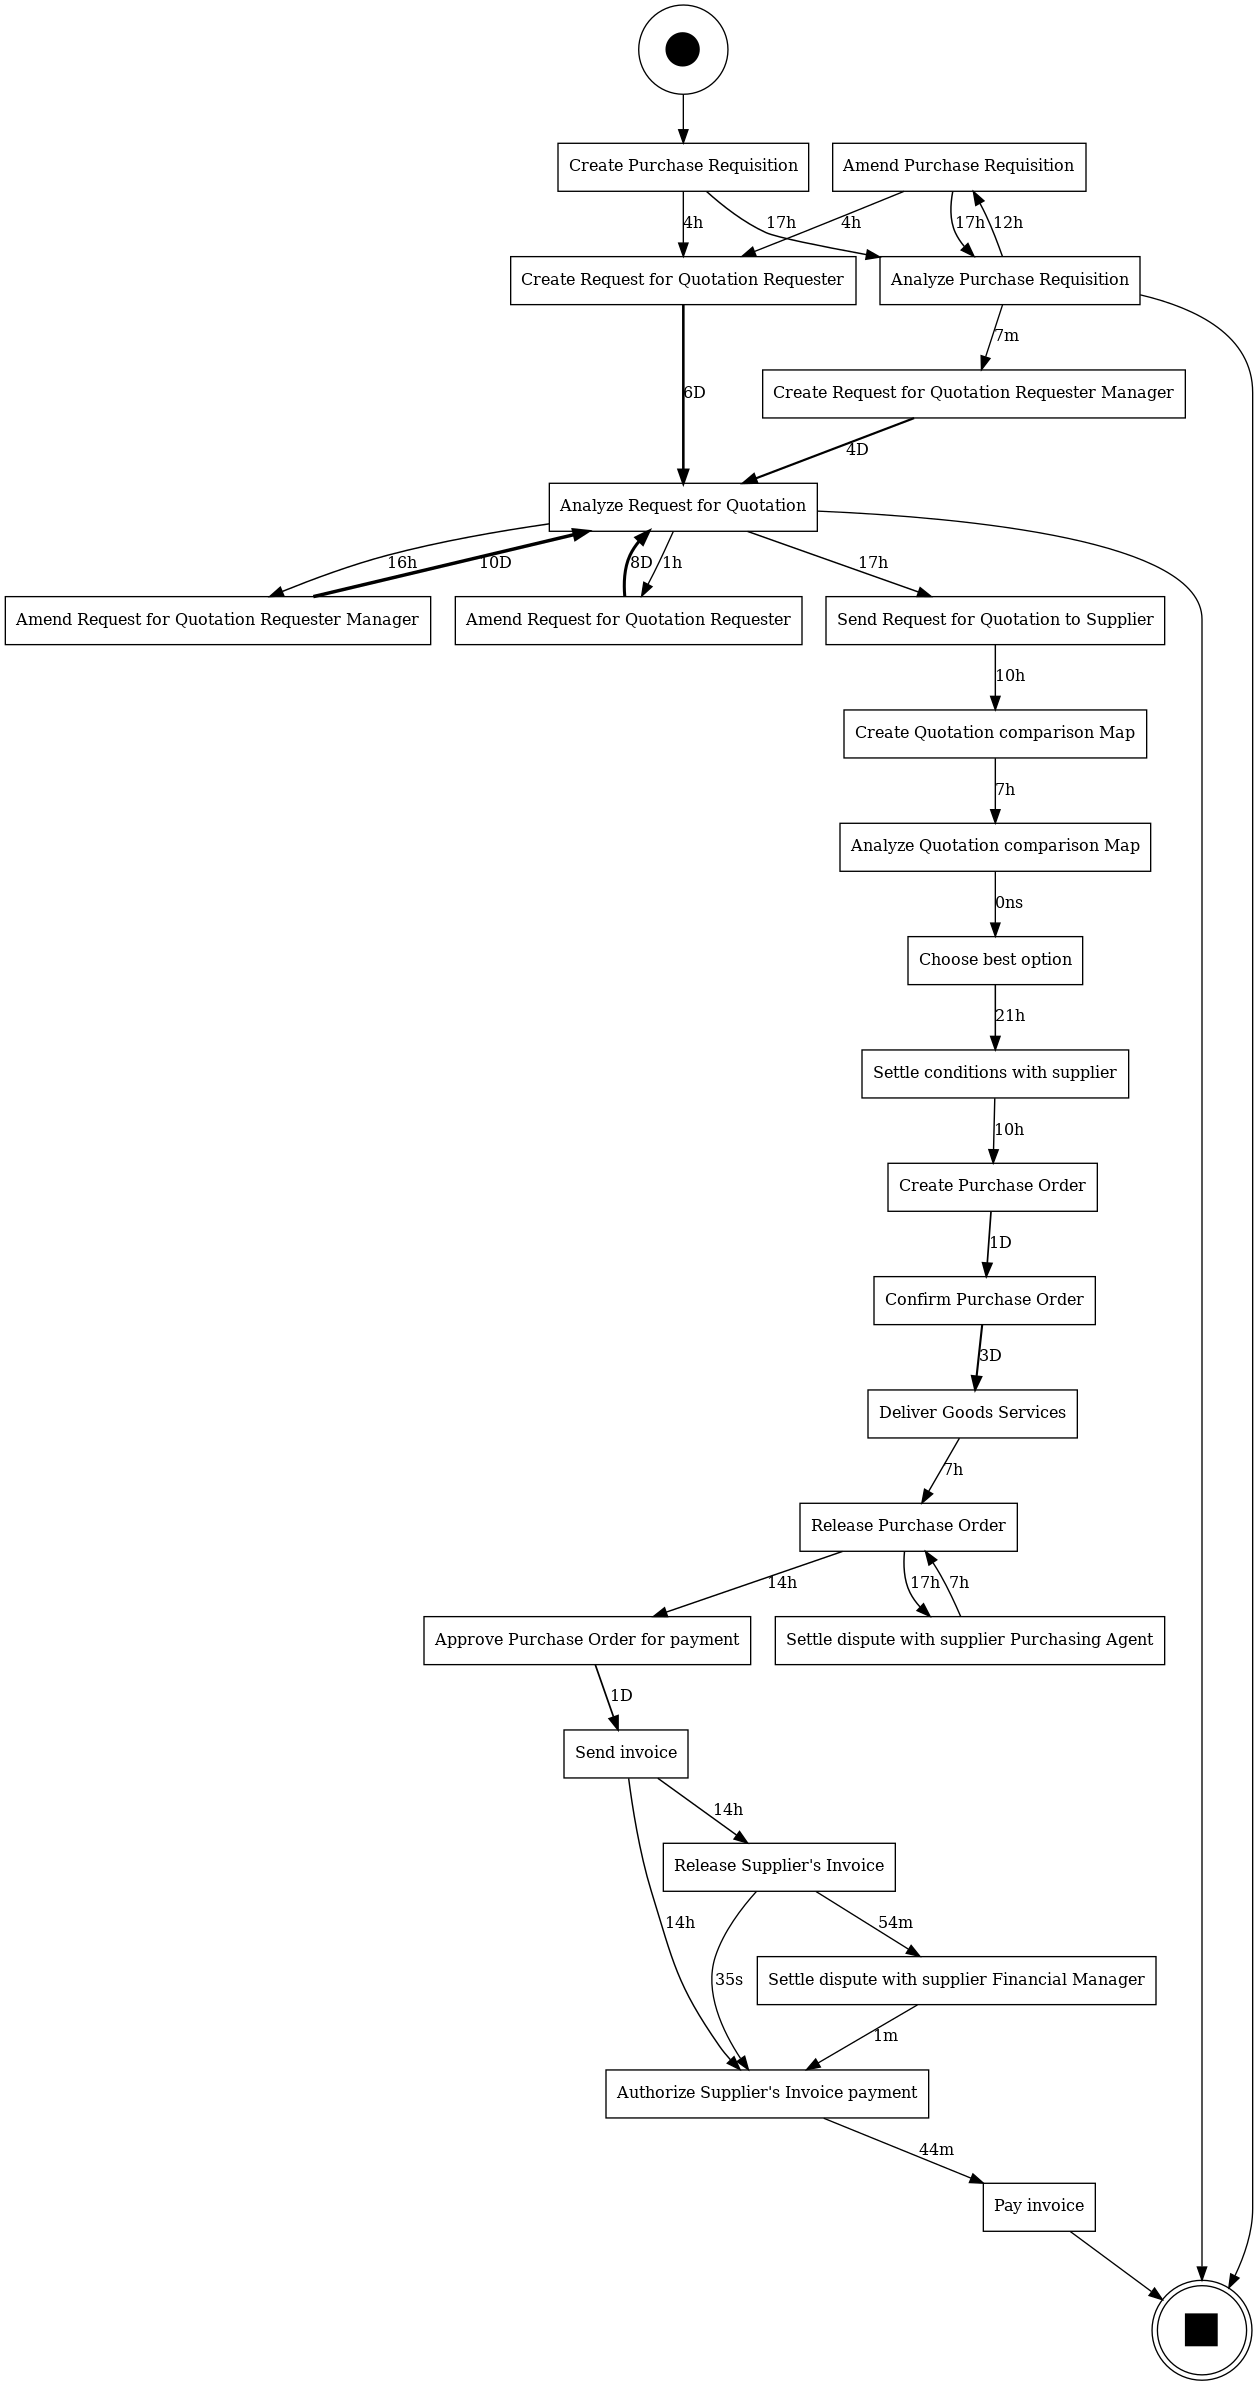
\includegraphics[width=.8\textwidth]{perfdfg.png}
\end{frame}

\begin{frame}[fragile]{Performance Mining --- Dotted Chart}
\begin{itemize}
   \item Identify batching of activities
   \item Identify different variants
   \item Case arrival and case finishing rates
\end{itemize}
\footnotesize
\begin{pythoncode}
pm4py.view_dotted_chart(log, show_legend=False)
pm4py.save_vis_dotted_chart(log, 
   'dottedchart.png', show_legend=False)
\end{pythoncode}
\end{frame}

\begin{frame}{Performance Mining --- Dotted Chart}
\centering
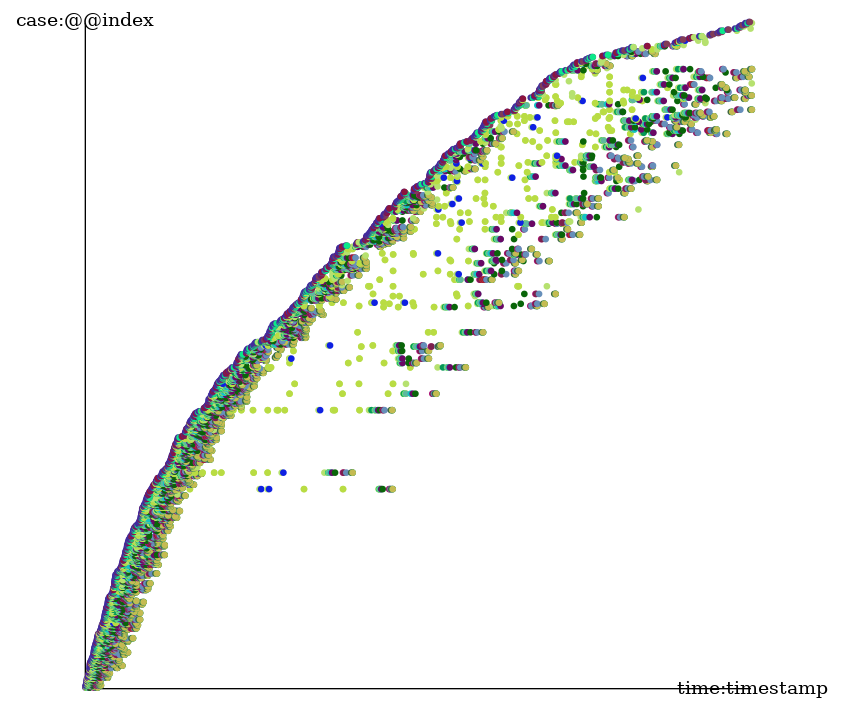
\includegraphics[width=.8\textwidth]{dottedchart.png}
\end{frame}

\begin{frame}[fragile]{Performance Mining --- Performance Spectrum}
\begin{itemize}
   \item Identify variations in wait times
\end{itemize}
\footnotesize
\begin{pythoncode}
pm4py.view_performance_spectrum(log,
    ['Send invoice', 'Pay invoice'])
pm4py.save_vis_performance_spectrum(log,
    ['Send invoice', 'Pay invoice'],
    'perfspectrum.png') 
\end{pythoncode}
\end{frame}

\begin{frame}{Performance Mining --- Performance Spectrum}
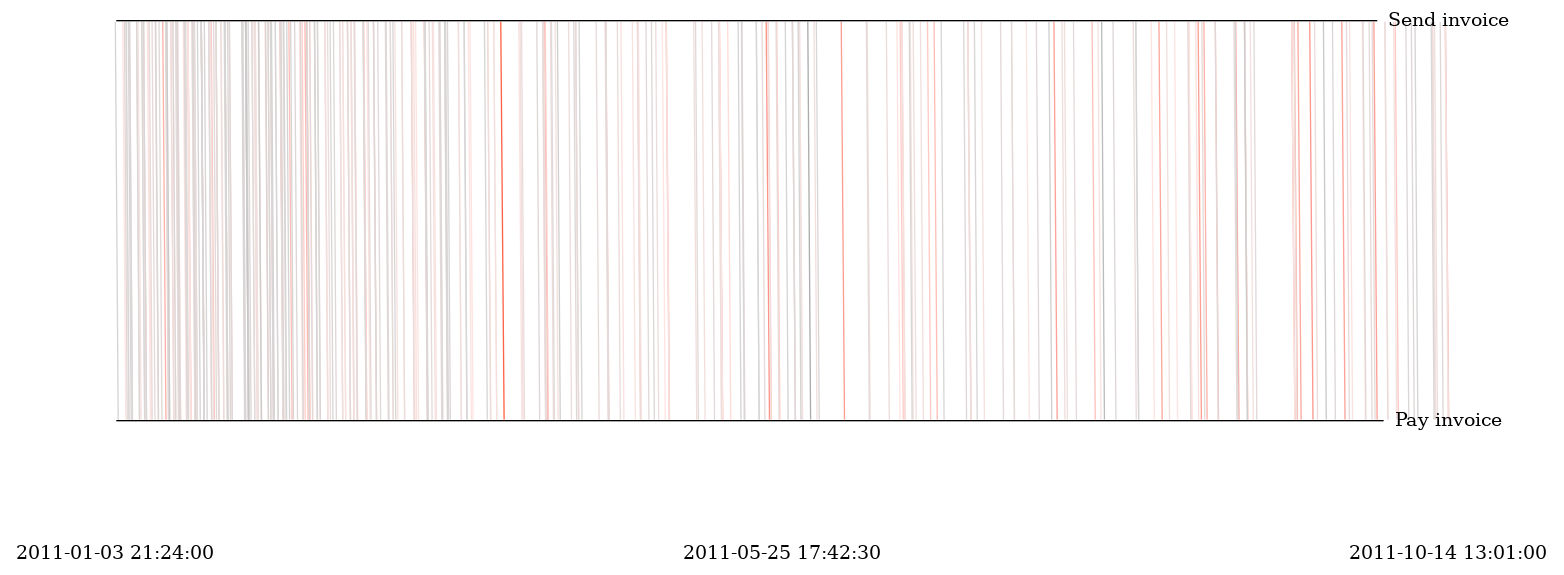
\includegraphics[width=\textwidth]{perfspectrum.png}
\end{frame}
    
\begin{frame}[fragile]{Performance Mining --- Event Distribution}
\begin{itemize}
   \item Identify distribution of when events/activities occur
\end{itemize}
\footnotesize
\begin{pythoncode}
pm4py.view_events_distribution_graph(log, 'days_week')
pm4py.view_events_distribution_graph(log, 'days_month')
pm4py.view_events_distribution_graph(log, 'months')
pm4py.view_events_distribution_graph(log, 'weeks')
\end{pythoncode}
\end{frame}

\begin{frame}{Performance Mining --- Event Distribution}
\centering
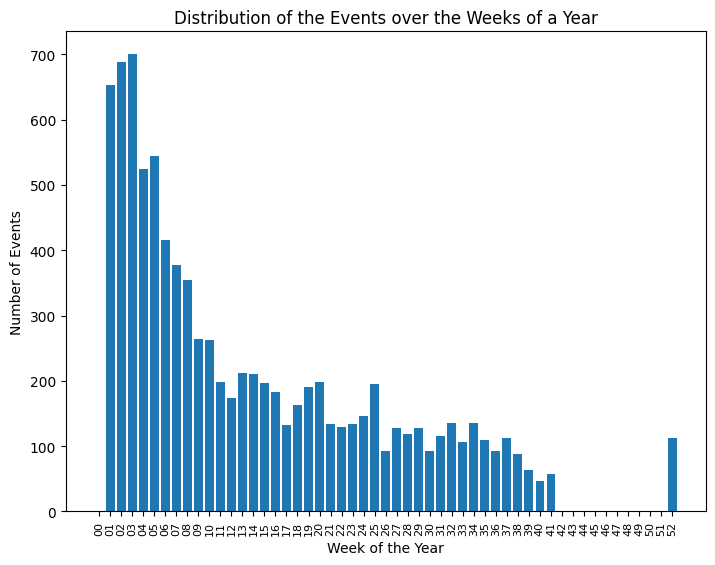
\includegraphics[width=.8\textwidth]{eventsdistribution.png}
\end{frame}

\begin{frame}[fragile]{Performance Mining --- Events per Time}
\footnotesize
\begin{pythoncode}
pm4py.view_events_per_time_graph(log)
pm4py.save_vis_events_per_time_graph(
    log, 'eventspertime.png')
\end{pythoncode}
\end{frame}

\begin{frame}{Performance Mining --- Events per Time}
\centering
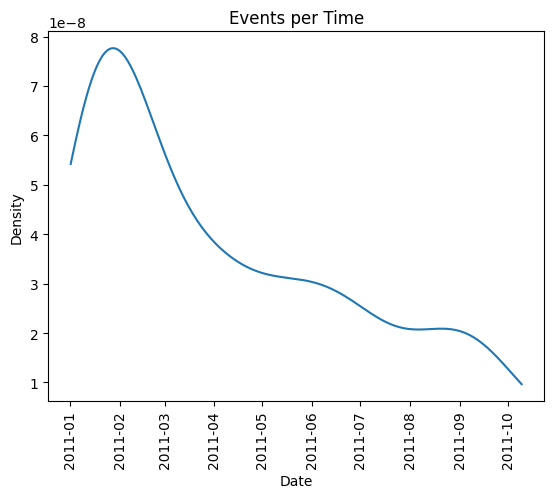
\includegraphics[width=.8\textwidth]{eventspertime.png}
\end{frame}


\begin{frame}[fragile]{Organizational Mining}
\begin{block}{Activity-Based Resource Similarity}
\begin{itemize}
   \item Identify similar resources based on the set of activities they perform
\end{itemize}
\end{block}
\footnotesize
\begin{pythoncode}
sna_graph = \
 pm4py.discover_activity_based_resource_similarity(log)

pm4py.view_sna(sna_graph, variant_str='networkx')
pm4py.view_sna(sna_graph, variant_str='pyvis')

pm4py.save_vis_sna(sna_graph, 'ressimilarity.png',
    variant_str='networkx')
\end{pythoncode}
\end{frame}

\begin{frame}{Organizational Mining \\ \small Activity-Based Resource Similarity}
\centering
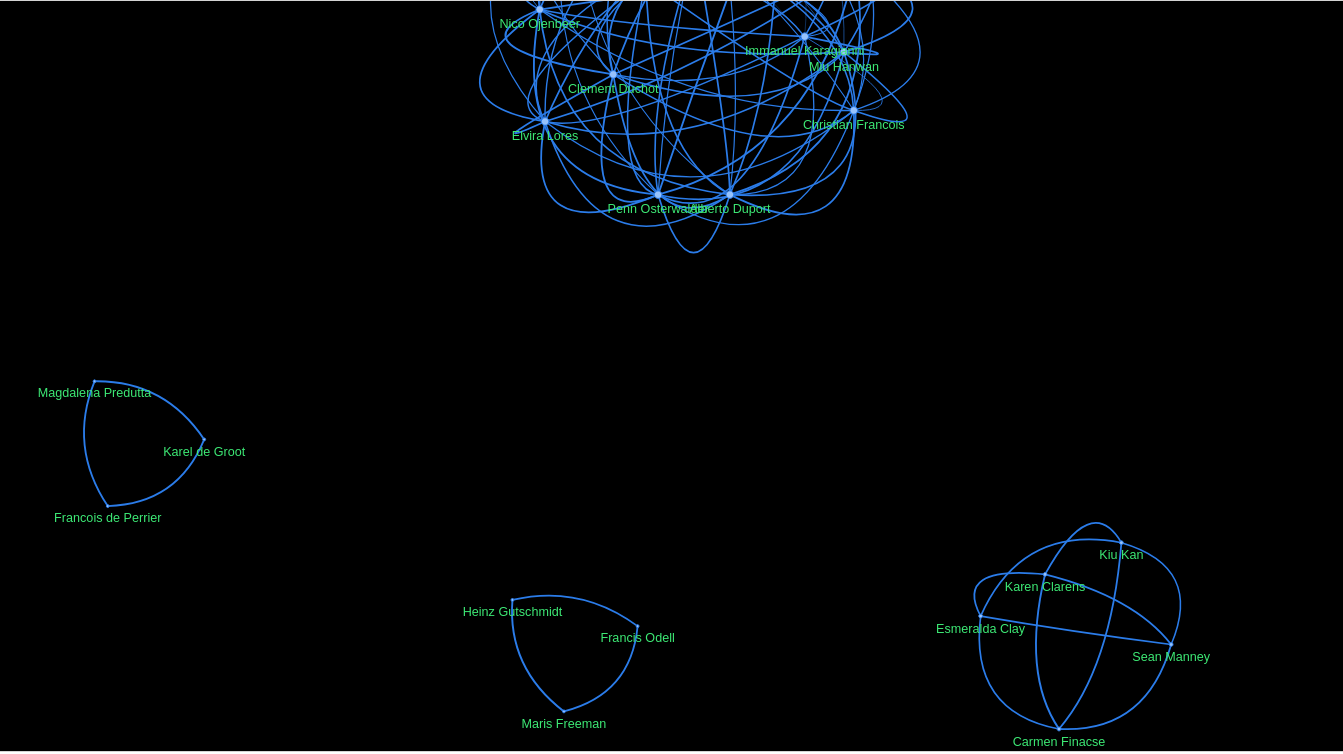
\includegraphics[width=.9\textwidth]{screen3.png}
\end{frame}

\begin{frame}[fragile]{Organizational Mining}
\begin{block}{Handover of Work Network}
\begin{itemize}
   \item Identify resources that pass work from one to another
   \item A DFG for resources instead of activities
\end{itemize}
\end{block}
\footnotesize
\begin{pythoncode}
dfg, start, end = pm4py.discover_dfg(log,
    activity_key='Role')
pm4py.view_dfg(dfg, start, end, rankdir='LR')

pm4py.save_vis_dfg(dfg=dfg,
    start_activities=start, 
    end_activities=end, 
    file_path='handover.png', rankdir='TB')
\end{pythoncode}
\end{frame}

\begin{frame}{Organizational Mining\\ \small Handover of Work Network}
\centering
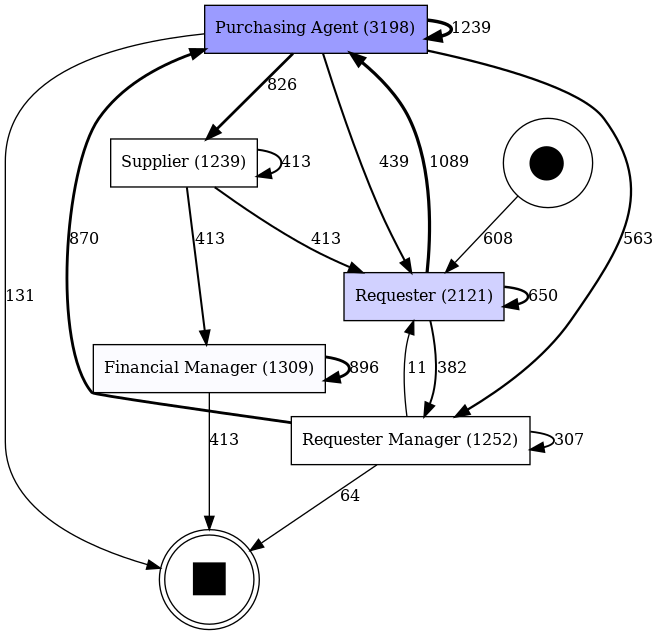
\includegraphics[width=.7\textwidth]{handover.png}
\end{frame}

\begin{frame}[fragile]{Organizational Mining}
\begin{block}{Organizational Roles}
\begin{itemize}
   \item Identify similar resources based on the set of activities they perform
\end{itemize}
\end{block}
\footnotesize
\begin{pythoncode}
roles = pm4py.discover_organizational_roles(log)
print(roles)
\end{pythoncode}
\end{frame}

\begin{frame}[fragile]{Organizational Mining}
\begin{block}{Working-Together Network}
\begin{itemize}
   \item Resources work together, if they collaborate on some trace
\end{itemize}
\end{block}
\footnotesize
\begin{pythoncode}
sna_graph = pm4py.discover_working_together_network(log,
   resource_key='Role')
pm4py.view_sna(sna_graph, variant_str='pyvis')   
pm4py.view_sna(sna_graph, variant_str='networkx')   
\end{pythoncode}
\end{frame}

\begin{frame}{Oganizational Mining \\ \small Working-Together Network}
\centering
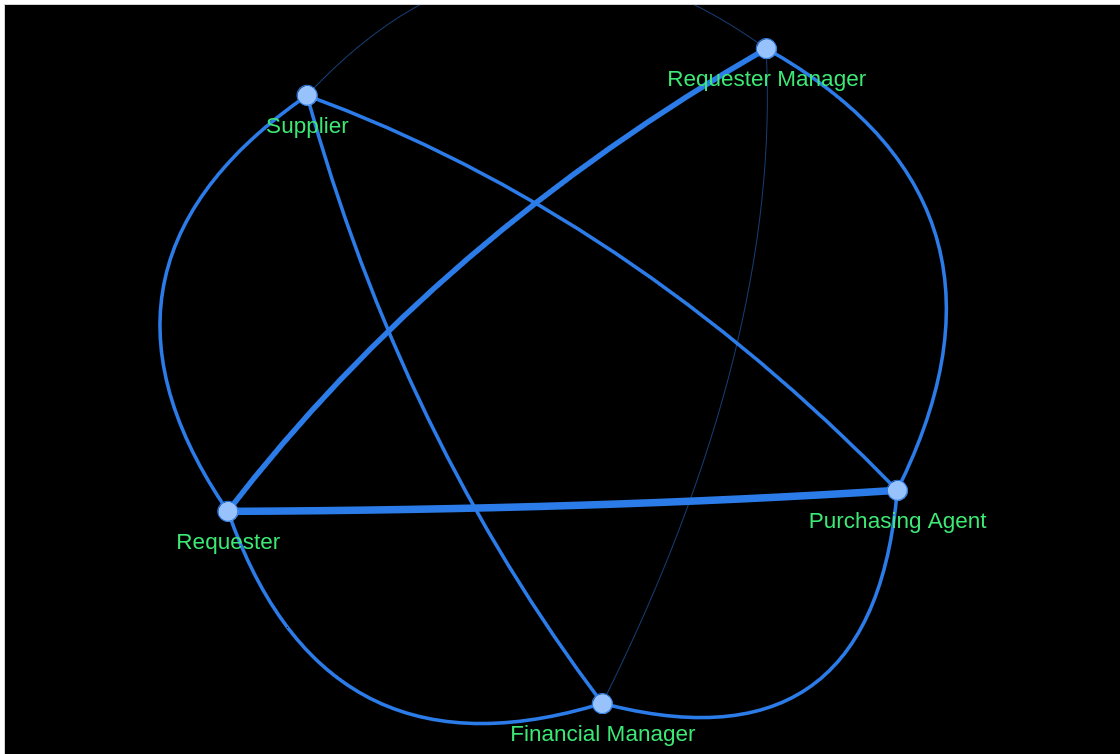
\includegraphics[width=.9\textwidth]{screen4.png}
\end{frame}

\end{document}
